\documentclass[11pt, oneside, listof=totoc]{scrbook}

\usepackage[english]{babel}
\counterwithout{figure}{chapter}

\usepackage[linear]{handout}
\usepackage{scrhack}
% \setlist{nosep}

%% Quantum Circuits %% 
\usepackage{qcircuit}

\usepackage{listings}

\definecolor{codegreen}{rgb}{0,0.6,0}
\definecolor{codegray}{rgb}{0.5,0.5,0.5}
\definecolor{codepurple}{rgb}{0.58,0,0.82}
\definecolor{backcolour}{rgb}{0.95,0.95,0.92}

\definecolor{identifiercolor}{rgb}{.4,.6,.56}
\definecolor{stringcolor}{gray}{0.5}
\definecolor{inactivecolor}{rgb}{0.15,0.15,0.5}

\lstdefinestyle{mystyle}{
    basicstyle={\fontfamily{fvm}\selectfont},
    backgroundcolor=\color{backcolour},   
    commentstyle=\color{codegreen},
    keywordstyle={\bfseries\color{inactivecolor}},
    stringstyle={\bfseries\color{stringcolor}},
    identifierstyle={\bfseries\color{identifiercolor}},
    numberstyle=\tiny\color{codegray},
    breakatwhitespace=false,         
    breaklines=true,                 
    captionpos=b,                    
    keepspaces=true,                 
    numbers=left,                    
    numbersep=5pt,                  
    showspaces=false,                
    showstringspaces=false,
    showtabs=false,                  
    tabsize=2
}

\lstset{style=mystyle}

\lstdefinestyle{Mathematica}{
morekeywords=[3]{KroneckerProduct, PauliMatrix, HadamardMatrix}
}

\renewcommand{\lstlistingname}{Code} % adjusts Listings caption and reference lst
\renewcommand{\lstlistlistingname}{List of Code Snippets}

%% EULER Fonts %%
% \usepackage[T1]{fontenc}
% \usepackage{textcomp}
% \usepackage{opensans}
% \usepackage[boldsans]{ccfonts}
% \usepackage[euler-digits]{eulervm}

%% Math Macros %%
\renewcommand{\H}{\mathcal{H}}
\renewcommand{\O}{\mathcal{O}}
\renewcommand{\HH}{\mathscr{H}} 

\renewcommand{\u}{\uparrow}
\renewcommand{\d}{\downarrow}
\renewcommand{\r}{\rightarrow}
\renewcommand{\l}{\leftarrow}

\newcommand{\ku}{\ket{\uparrow}}
\newcommand{\kd}{\ket{\downarrow}}
\newcommand{\kr}{\ket{\rightarrow}}
\newcommand{\kl}{\ket{\leftarrow}}

\newcommand{\UU}{\mathcal{U}}

%% Image Path %%
\graphicspath{{images/}}

%% TOC Setup %%
\setcounter{tocdepth}{3}
\setcounter{secnumdepth}{3}

\title{Quantum Cellular Automata}
\subtitle{NIUS Physics (Batch 20) \\ Mid-Term Report \\ Camp: 20.2}
\author{
    Piyush Kumar Singh\thanks{\mailto{pks22ms027@iiserkol.ac.in}} \\ {\large IISER Kolkata} 
    \and
    % Rhythm Anand\thanks{\mailto{rhythm.anand@students.iiserpune.ac.in}} \\ {\large IISER Pune}
    % \and
    Sambuddha Sanyal\thanks{\mailto{sambuddha.sanyal@iisertirupati.ac.in}} \\ {\large IISER Tirupati}
}
\date{
    \today \\[3ex]
    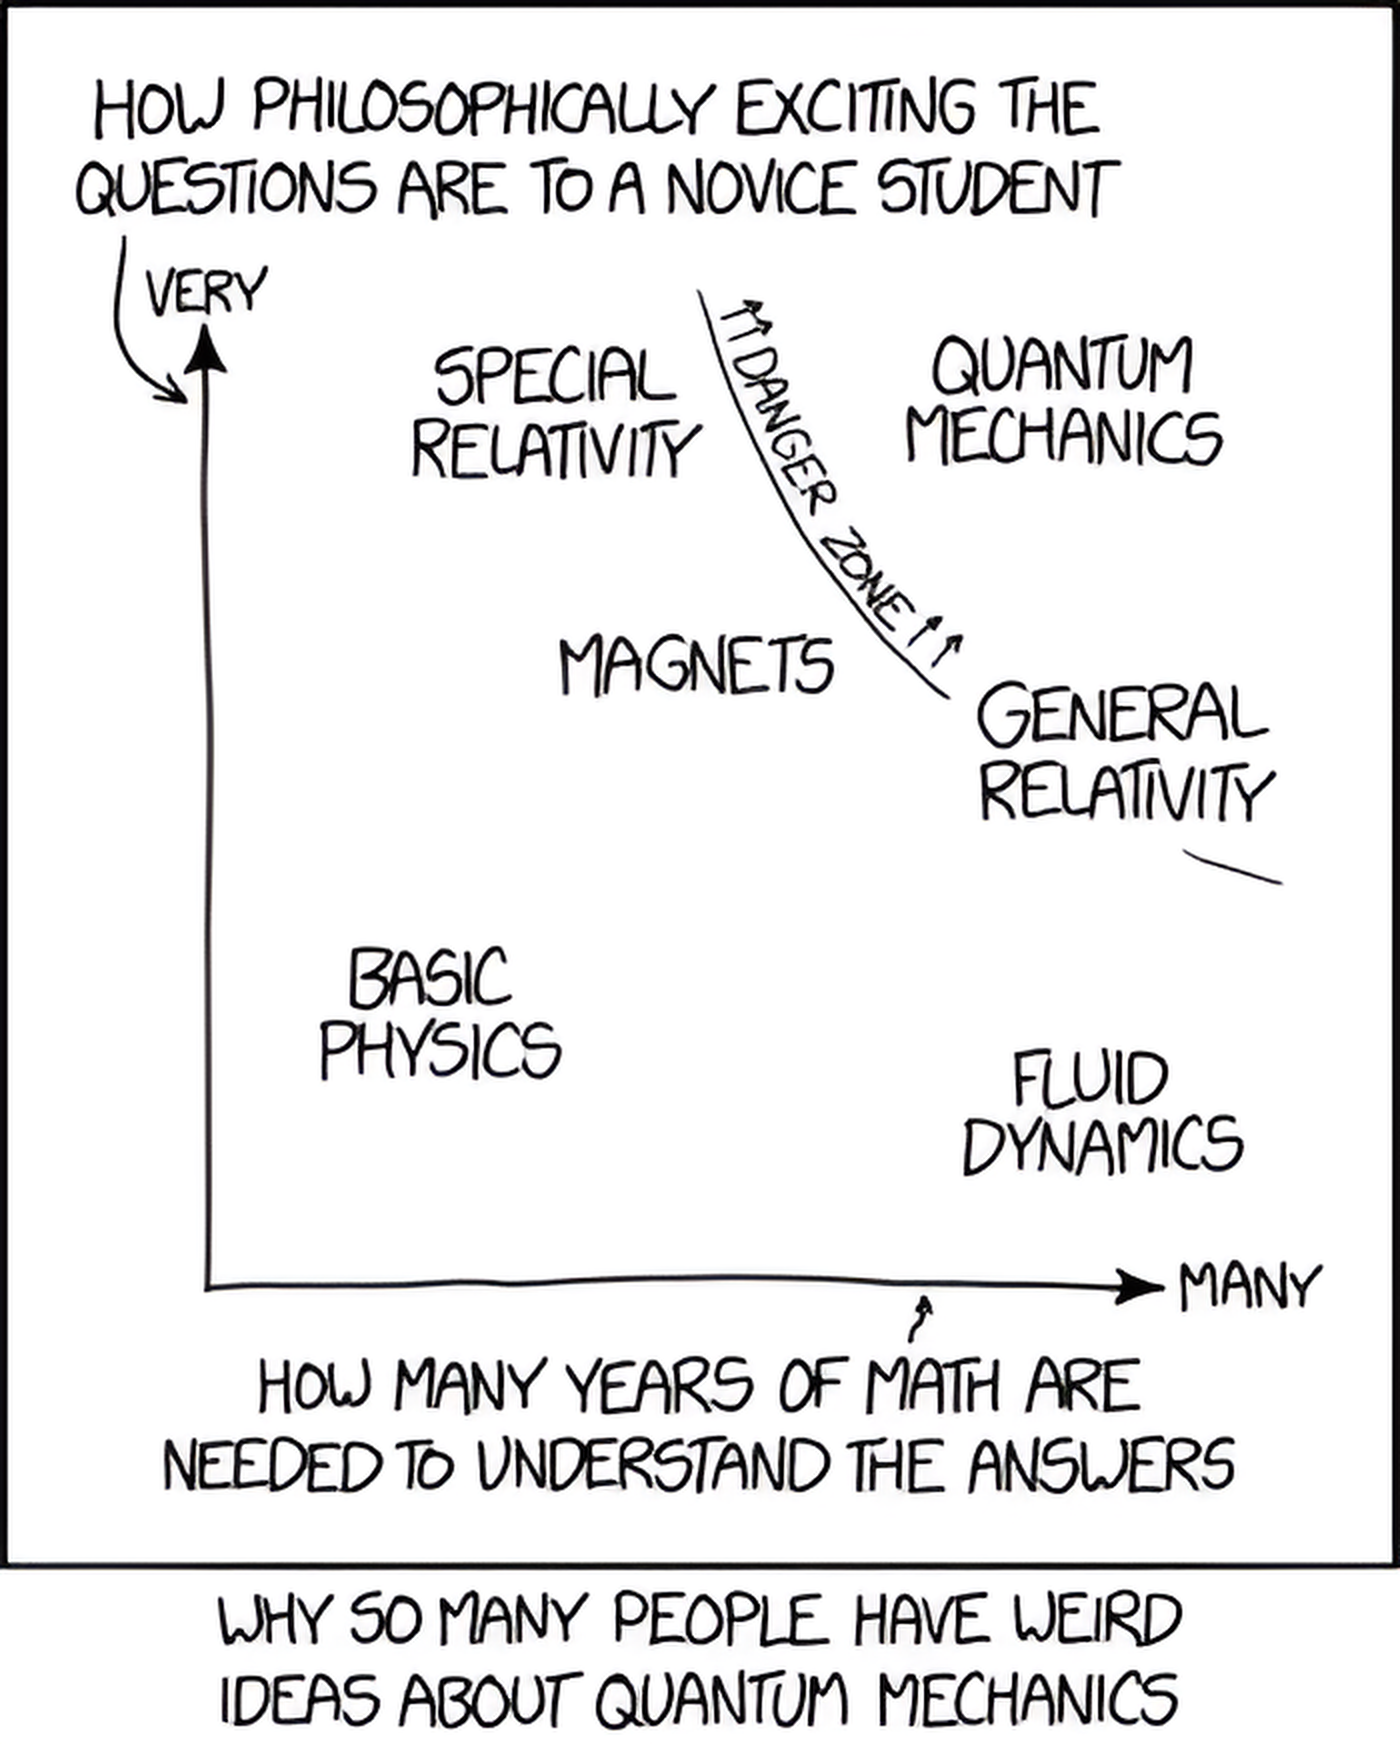
\includegraphics[width = 0.7\textwidth]{quantum-xkcd-better.png}
}

\changemaincolor{Emerald}
\changesecondcolor{Periwinkle}

% \usepackage{biblatex}
\addbibresource{references.bib}

\hypersetup{
    pdftitle={Quantum Cellular Automata},
    pdfauthor={Piyush Kumar Singh, Sambuddha Sanyal},
    pdfkeywords={physics, cellular automata, quantum cellular automata, thermalization},
    linktocpage=true
}

\begin{document}
\frontmatter
\begin{titlepage}
    \let\newpage\relax%
    \singhtitle
\end{titlepage}

\chapter*{Acknowledgement}
\addcontentsline{toc}{chapter}{Acknowledgement}

{\large\noindent
    This work was supported by the National Initiative on Undergraduate Science (NIUS) undertaken
    by the Homi Bhabha Centre for Science Education, Tata Institute of Fundamental Research
    (HBCSE-TIFR), Mumbai, India. We acknowledge the support of the Department of Atomic
    Energy, Govt. Of India, under Project Identification No. RTI4001.\\

    Special appreciation is extended to my project instructor, Sambudhha Sanyal, for his guidance, expertise, and unwavering commitment throughout this project. His mentorship has been instrumental in shaping the direction and success of our research endeavors. We are truly grateful for his dedication and encouragement, which have significantly enriched our learning experience within the framework of the NIUS program.
}

\tableofcontents
\lstlistoflistings

\mainmatter

\chapter{Introduction}

% \lipsum[1]\cite{Hadeler2017}

Cellular automata are discrete mathematical models used to simulate complex systems. John von Neumann first introduced the concept \cite{Neumann1966} in 1966. In 1970, an article written by Martin Gardner \cite{Gardner1970} introduces us to a compelling use case of this abstract concept, ``The Game of Life,'' invented by J. H. Conway.

% In classical cellular automata, the system is divided into discrete cells arranged in a grid. Each cell can be in one of a finite number of states. The state of a cell is typically updated over discrete time steps according to a set of rules based on the states of its neighbouring cells.

In a conference in 1982, R. P. Feynman expressed his view (or dream) of using `Quantum Physics' in computers \cite{Feynman1982} to simulate complex physical systems using the idea of density matrix (proposed by Neumann in 1955 \cite{Neumann2018}); building on his idea Feynman introduced the world to a weird collaboration named ``Quantum Cellular Automata'' (QCA) in an article published in 1986 \cite{Feynman1986}.

And there are multiple reasons why we should care about QCAs. First, this is part of a broad field of `Quantum Information Processing,' any development in QCA may help us understand how we can harness quantum properties for computation. Second, the classical systems exhibit some new emergent behaviors, so we want to know if we can also have these emergent behaviors in QCAs.

% When this abstract concept is combined with seemingly weird notions of `Quantum Mechanics,' we get Quantum Cellular Automata (QCA).

Also, in the later part of the discussion, we will see the application of these `discrete' quantum systems (in the form of ``\impt{Random Quantum Circuits}''\cite{Fisher2023}), explaining some of the various emergent properties like:
\begin{enumerate}[(a), noitemsep]
    \item Periodic Fidelity,
    \item Information spread (encoded as \emph{Operator Spread}).
\end{enumerate}

\section{Cellular Automata}

A cellular automaton (CA) is a group of ``coloured'' cells on a predetermined-shaped grid that follows a set of rules depending on nearby cell states to evolve over many discrete time steps. After that, the rules are applied repeatedly for as many time steps as needed.

It turned out that reaction-diffusion systems, biological pattern development, fluid flows, and traffic models are only a few real-world uses for CAs. Lattice gas cellular automata are a specific type of CA used to simulate fluid dynamics. The Navier-Stokes equation can be obtained by selecting the appropriate model. Lattice Boltzmann models have taken their place, using continuous functions at the lattice locations rather than discrete variables. More aspirationally, CAs have been proposed as discrete physics models with many desirable characteristics, such as dynamical homogeneity and localization. But, while this is a fascinating idea, physics is ultimately quantum, and CAs cannot adequately represent, e.g., Bell inequality violation, which occurs from quantum entanglement.

Before giving a formal definition, let's look at an example:
\begin{example}[Rule Number 110]
    \label{eg:rule110}
    Consider a one-dimensional array of bits (\ie cells having two states, namely `0' or `1'). The update rule of a bit is dependent on the initial state of that bit as well as the state of its neighbouring bits. The rule can be summarized as follows:
    \begin{table}[H]
        \centering
        \begin{tabular}{ | c | c | c | c | c | c | c | c | c | }
            \hline
            Initial state of a bit and its neighbours & 111 & 110 & 101 & 100 & 011 & 010 & 001 & 000 \\
            \hline
            New state of middle bit                   & 0   & 1   & 1   & 0   & 1   & 1   & 1   & 0   \\
            \hline
        \end{tabular}
        \caption{Update rule for a \textit{one}-dimensional CA}
        \label{tab:rule110}
    \end{table}
    We named this update rule as \verb|Rule 110| because if you treat the last row of the table as a binary number, it converts to 110 in the decimal system. This CA can simulate a Turing machine efficiently (with only polynomial overhead).
    \begin{figure}[H]
        \centering
        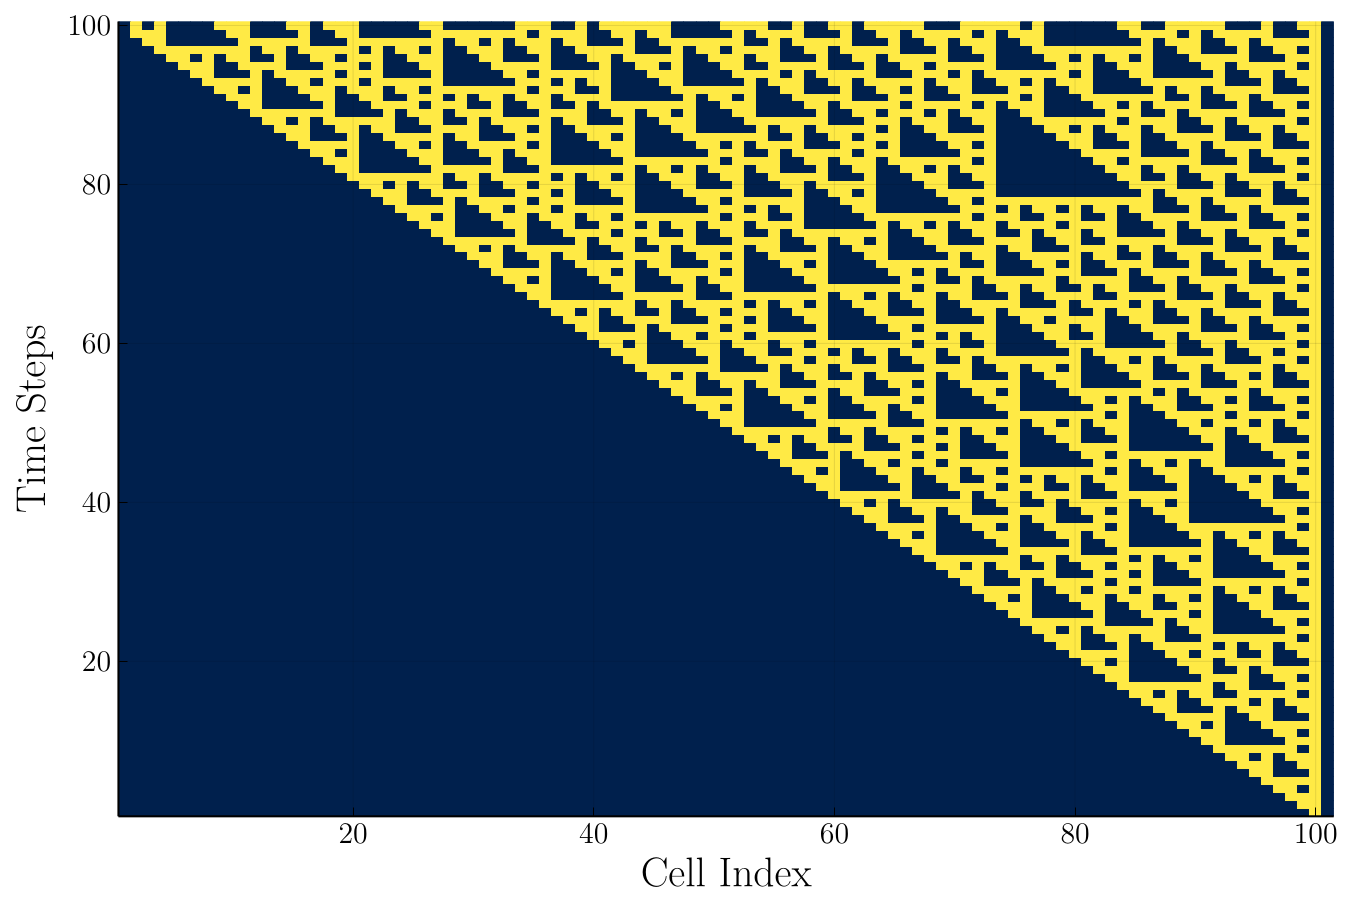
\includegraphics[width = 0.7\textwidth]{rule110_cellular_automaton.png}
        \caption{An example of a CA evolution for the rule 110 CA, with time going up. Bits with value 1 are
            represented by the yellow squares, while blue squares represent 0.}
        \label{fig:rule110}
    \end{figure} \noindent

\end{example}

\begin{definition}[Cellular Automata]
    A Cellular Automaton is a 4-tuple \(\qty(L, \Sigma, \mathcal{N}, f)\) consisting of a $d$-dimensional lattice of cells indexed by integers, $L = \Z^d$, a finite set $\Sigma$ of cell states, a finite neighbourhood scheme $\mathcal{N} \subseteq \Z^d$, and a local transition function $f: \Sigma^{\mathcal{N}} \to \Sigma$.
\end{definition}

% There are a few unique characteristics of this local transition function \(f\). Consider a cell \(x \in L\)
To better understand this local transition function \(f\), consider a cell \(x \in L\). This function takes the state of the neighbours of \(x\) as the argument, which is indexed by the set \(\mathcal{N}\) at the current time \(t \in \Z\) to spit out the state of cell $x$ at time $t + 1$.

\noindent This observation points us towards two important properties of cellular automata that will help us understand why CAs are very helpful in simulating certain systems:

\begin{itemize}
    \item cellular automata are \vocab{space-homogeneous} \ie the local transition function performs the same function at each cell.
    \item Also, cellular automata are \vocab{time-homogeneous} \ie the local transition function does not depend on the current time $t$.\footnote{We will review these properties in detail in \cref{ssec: locality,ssec: universality}}
\end{itemize}

\noindent We can define the current state of the lattice (or CA) as a \emph{configuration} \(C \in \Sigma^{L}\), which has the information about the state of each cell at time \(t\). Now, using this idea, we can define a `\emph{global}' transition function \(F: \Sigma^{L} \to \Sigma^{L}\), which acts on the entire latter rather than on individual cells and spits out another configuration \(C'\) for the lattice at time \(t+1\).

\begin{remark}[Revisiting Rule 110]
    Observe the \cref{eg:rule110}; we can fit this scenario in the definition. In this case \(L = \Z\), \(\Sigma = \qty{0, 1}\), for $i^{\text{th}}$ cell \(\mathcal{N} := \qty{i-1,~ i,~ i+1}\) and \(f\) is defined according to the update rule specified in \cref{tab:rule110}.
\end{remark}

\pagebreak
\subsection{Characteristics of Cellular Automata}

In the definition and example, we have used a few terms; now we will define them (and these will be the main characteristics of cellular automata):
\begin{list}{}{}
    \item[\bfseries Discrete Space-Time:] In our discussion, we have defined the lattice \((L)\) to be \(d\)-dimensional integer space, which makes our area of interest a discrete space. Our evolution to the next state is also discrete since we evolve our states from \(t \to t+1\) (or predefined time steps).

    \item[\bfseries Finite State Set:] The set \(\Sigma\) is finite \ie every cell has only finitely many states of being in. Generally, in classical systems, we have state set \(\Sigma = \qty{0, 1}\), also called `binary cellular automata.'

    \item[\bfseries Cell/Cell-state:] Every space-position vector \(i \in L = \Z^d\) identifies a cell which contains a cell-state \(c_i \in \Sigma\).

    \item[\bfseries Configuration:] A configuration \(C\) is the concatination of all cell-states over the entire lattice \(L\) at a given time \(t\) which means that every configuration is an element of set \(\Sigma^L\).

    \item[\bfseries Local Transition Function:] We know time is also discrete in our system (with a predefined time step). We use a local transition function \(f\) that defines the state of every cell after each time evolution. We refer to this function as a local function, as it only takes the states of the `neighbouring' cells as an argument.

    \item[\bfseries Neighbourhood Scheme:] As we have defined, the outcome of our local function at any cell \(i\) depends on the set of cell-states of neighbouring cells. This set is defined by the neighbourhood scheme \(\mathcal{N}\) on cellular automata.

    \item[\bfseries Global Function:] For a given lattice \(L\) (with a defined neighbourhood scheme), the local transition function \(f\) imposes a global transition function \(F\) on the set of all possible configurations. This global function determines the \emph{space}/\emph{time} behavior of the cellular automaton on an initial configuration.
\end{list}

\subsection{Locality} \label{ssec: locality}

% The word locality has a defined meaning in day-to-day conversations, but here, this locality means something more than that. 
In physics, locality implies we are talking about the \impt{Principle of Locality}, which states that \uline{an object is influenced directly only by its immediate surroundings}. If a theory that includes this principle is said to be a ``local theory.'' This idea of locality evolved from the classical field theory; building upon this idea, if an event at a point is cause for an effect at another point, a wave or a particle must travel through space-time between the two points, carrying the influence.

Einstein postulated that causal influence couldn't be transmitted between two points faster than the speed of light \(c\), in the \vocab{Special Theory of Relativity}, which means that if two points are spacelike separated, they can't influence each other. % This limit on speed also relates to the locality and causality

In the context of cellular automata, we know that the state of a cell is only influenced by the states of finite neighbours (decided by neighbourhood scheme). Since the state of any cell is influenced by its surroundings, we can say that the cellular automata theory is local.
\subsection{Universality} \label{ssec: universality}
% \lipsum[3]

\section{Quantum Cellular Automata}
R. P. Feynman introduced the idea of Quantum Cellular Automata with a vision that it can be used to simulate `Quantum Physics' as we don't have a classical analog of many quantum phenomena. In \cite{Watrous1995}, he has proven that QCAs are an alternative paradigm of quantum computers. They have shown QCAs to be universal, implying they could efficiently simulate a quantum Turing machine.

This demonstration showed that QCAs are very important for quantum computers, so many have tried to formulate a theory. But there was an enormous challenge in front of the scientists: after some local function has updated one cell, we will lose the information about the state of the cell at time \(t\) as we require it for updating other cells. So somehow, we have to clone the state of this cell to some other cell, but by the \vocab{no-cloning theorem}, it is simply impossible.


\chapter{Random Quantum Circuits}

As we know, discrete quantum circuits are good examples of QCAs. In \cite{Fisher2023}, they have extended this idea of quantum circuits as QCAs to incorporate an element of randomness into the local unitary gates (or operations). They also included measurements of quantum circuits (which are irreversible and non-local). This kind of quantum circuit is known as ``Random Quantum Circuit (RQC).''

This discussion will use a simple discrete-time model for many-body quantum systems. This model's lattice of spins (qubits) evolves by applying local unitary gates and projective measurements. This discrete-time structure can be seen as an example of `\vocab{Totterization}' of a continuous-time Hamiltonian evolution \(\qty[\ie ~ e^{i \hat{H} t / \hslash}]\), assuming the time-step to be finite \(\qty(\ie ~ t \in \Z)\), which also implies that energy is not conserved in this approach.

\section{Methodology}

In this section, we will construct the system used in this analysis. And also go through some of the mathematical tools required to understand ``\impt{Quantum Entanglement}.''

\subsection{Defining System}
Let a \(d\)-dimensional lattice \(L = \Z^{d}\) composed of qubits (or in general \(q\)-level systems ``\vocab{qubits}'') which represents a \(d\)-dimensional quantum many-body system arranged in a spatially local manner. The discrete-time evolution of such a quantum many-body system by applying local unitary gates defines a quantum circuit. We will restrict our discussion to
\begin{enumerate}[(i), noitemsep]
    \item local quantum gates -- unitary transformation acting on a few neighbouring qubits,
    \item local projective measurements -- observations which leave the measured qubit in a state with definite eigenvalue of the measured operator.
\end{enumerate}

\subsection{Quantum Entanglement}

In 1935 \cite{Einstein1935}, Albert Einstein, Boris Podolsky, and Nathan Rosen published a paper on counterintuitive predictions that quantum mechanics makes for pairs of objects prepared together in a particular way. In this study, the three formulated a thought experiment (today known as EPR-paradox) to show that ``the quantum-mechanical description of physical reality given by wavefunctions is not complete.''

\begin{definition}[Quantum Entanglement]
    An entangled system is one whose quantum state cannot be separated as a tensor product of the quantum states of its local constituents.
\end{definition}

Consider two arbitrary quantum many-body systems $A$ and $B$, with respective Hilbert spaces \(\H_{A}\) and \(\H_{B}\). The composite Hilbert space is a tensor product given by \(\H:= \H_{A} \otimes \H_{B}\). Say system \(A\) is in a state \(\ket{\Psi}_A\) and \(B\) is in \(\ket{\Psi}_B\), the state of the composite system is given by \(\ket{\Psi}_A \otimes \ket{\Psi}_B\).
\begin{remark}[Pure and Entangled state]
    If the state of the composite system can be expressed in the tensor product of the states of individual systems, then we call this composite state a separable state or \vocab{pure state}.

    \noindent Not all states are pure states. Let \(\qty{\ket{\mu}_A}\) be a set of basis for the space \(\H_A\) and set \(\qty{\ket{\nu}_B}\) be a basis for the space \(\H_B\). The most general state in \(\H\) is of the form
    \begin{equation}\label{eq:tensor_state}
        \ket{\Psi} = \sum_{\mu,\!\nu}^{} c_{\mu \nu} \ket{\mu}_A \otimes \ket{\nu}_B
    \end{equation}
    This state is separable if and only if there exist vectors \(\qty[c_{\mu}^{A}]\) and \(\qty[c_{\nu}^{B}]\) such that \(c_{\mu \nu} = c_{\mu}^{A} c_{\nu}^{B}\), yielding \(\ket{\Psi}_A:= \sum_{\mu} c_{\mu}^{A} \ket{\mu}\) and \(\ket{\phi}_B:= \sum_{\nu} c_{\nu}^{B} \ket{\nu}\). And it is inseparable if such vectors do not exist. If a state is inseparable, it is called an `\vocab{entangled state}.'
\end{remark}

\subsubsection{Density Matrix}

The density matrix language provides a convenient way to describe quantum systems whose state is unknown.
\begin{definition}[Density Matrix]
    Suppose a quantum system is in one of several states \(\ket{\Psi_i}\), with respective probabilities \(p_i\). We define \(\qty{p_i, \ket{\Psi_i}}\) an \emph{ensemble of pure states}. The density matrix can be defined as follows for this quantum system
    \[
        \rho \equiv \sum_{i} p_i \ket{\Psi_i} \bra{\Psi_i}
    \]
\end{definition}
{\bfseries Properties of density matrix:}
\begin{itemize}[noitemsep]
    \item \(\rho\herm = \rho\)
    \item \(\Tr\rho = 1 \quad \implies \quad \sum_{i} p_i = 1\)
    \item \(\Tr \rho^2 \le 1 \quad (\text{equality holds for a pure ensemble})\)
\end{itemize}
{\bfseries \uline{Reduced Density Function:}}\\
Consider a quantum many-body system composed of \(N\) qubits and defined by a wavefunction \(\ket{\Psi}\), which is bipartitioned into a subset of spins \(A\), with Hilbert space dimension \(D_{A}\), and its complement \(\bar{A}\), with Hilbert space dimension \(D_{\bar{A}}\).

Generally, there is no way to associate a pure state to a sub-system $A$. However, associating a density matrix with this sub-system is still possible. Let \(\rho_{T} = \ket{\Psi} \bra{\Psi}\) which is the projection operator onto this composite state. The density matrix for sub-system \(A\) is defined as a \vocab{partial trace} of \(\rho_T\) over the basis \(\qty{\ket{\nu}}\) of sub-system \(\bar{A}\):
\begin{equation}
    \rho_A := \sum_{\nu} \qty(\I{A} \otimes \bra{\nu}_{\bar{A}}) \qty(\ket{\Psi} \bra{\Psi}) \qty(\I{A} \otimes \ket{\nu}_{\bar{A}}) = \Tr_{\bar{A}} \ket{\Psi} \bra{\Psi}
\end{equation}
where, \(\I{A}\) is the identity operator in Hilbert space \(\H_A\). \(\rho_A\) is also referred to as \emph{reduced density matrix} of \(\rho_T\) on sub-system \(A\), encodes all operator expectation values solely within region $A$.

\subsubsection{Entanglement Entropy}

\begin{definition}[Entanglement Entropy]
    The entanglement entropy measures the degree of quantum entanglement between two subsystems constituting a two-part composite quantum system.
\end{definition}
Continuing the discussion of \(N\) qubits system, which has been bipartite into two sub-systems \(A\) and \(\bar{A}\).
There are multiple ways to define entanglement entropy for these two sub-systems; a few of them are listed below:
\begin{list}{}{}
    \item[\uline{von Neumann Entropy:}] For a bipartite system, von Neumann entropy \(S\) is defined as follows:
        \begin{equation}
            S_{A} = - \Tr(\rho_{A} \ln \rho_{A}) = - \Tr(\rho_{\bar{A}} \ln \rho_{\bar{A}}) = S_{\bar{A}}
        \end{equation}

    \item[\uline{\(n^\text{th}\) R\'enyi Entropy:}] \(S_{A}^{(n)} = \ln(\Tr \rho_{A}^n) / (1 - n)\), and as \(n \to \infty\), \(S_A^n \to S_A\) \ie the von Neumann entropy.
\end{list}


\section{A four-qubit example of RQC}

In this section, we will see what a local unitary operator is in light of quantum circuits and what a projective measurement is. Then, we will work out a discrete-time evolution of a four-qubit system under this local unitary operator and projective measurement numerically.

\subsection{Basics of Quantum Computer -- for a single qubit}
For a single qubit, we have a finite state space \(\Sigma = \qty{0, 1}\), so we can infer that Hilbert space \(\H\) for this system is 2-dimensional. The state set can be seen as eigenvalues of a Hermitian operator (to be precise, a Pauli matrix) \(Z\). With these assumptions, we can define the eigenbasis for this Hilbert space \(\H\) as
\[
    \B_Z = \qty{\ket{0} = \ku = \mqty(1 \\ 0), \ket{1}= \kd = \mqty(0 \\ 1)}
\]
This basis set is sometimes referred as ``\emph{computational basis}.'' Similarly, we can define the other two sets of eigenbasis corresponding to the two remaining Pauli matrices.
\begin{equation}
    \B_X = \qty{\ket{+} = \kr = \frac{1}{\sqrt{2}} \qty(\ku + \kd), \ket{-} = \kl = \frac{1}{\sqrt{2}} \qty(\ku - \kd)}
\end{equation}
In general, the time evolution of a quantum system (which is described by a wavefunction \(\ket{\Psi}\) at time \(t = 0\)) under a given Hamiltonian \(\mathscr{H}\) which is represented by a matrix \(\O\) is provided by
\[
    \ket{\Psi (t)} = \UU(t) \ket{\Psi}, \qquad \UU(t) := \exp(- i \O \frac{t}{\hslash})
\]
For a single qubit, all possible Hamiltonians are \(2 \times 2\) Hermitian operator, which can be written as a linear combination (over \(\R\)) of the three ``\vocab{Pauli Matrices}'' and the identity matrix. Define \(S = \qty{\I{}, X, Y, Z}\)
\begin{equation}
    X = \mqty(0 & 1 \\ 1 & 0), \qquad Y = \mqty(0 & -i \\ i & 0), \qquad Z = \mqty(1 & 0 \\ 0 & -1), \qquad \I{} = \mqty(1 & 0 \\ 0 & 1).
\end{equation}
Using this construction, we can decompose any Hamiltonian operator \(\O\) as
\[
    \O = \sum_{S} c_S S = c_{\I{}} \I{} + c_X X + c_Y Y + c_Z Z
\]
the coefficients in this expansion are real and given by \(c_S = \half \Tr(S \O)\). The corresponding unitary can be written as
\[
    u = \exp(- i \sum_{S} h_S S)
\]
where, the coefficients \(h_S\) are real.\\
{\bfseries \uline{Hadamard Gates:}} This gate is often referred as ``superposition gate'', and represented as \(H\) in quantum circuits. It maps the computational basis as follows:
\begin{equation*}
    \ku \xmapsto{H} \frac{\ku + \kd}{\sqrt{2}} = \kr \quad ; \quad \kd \xmapsto{H} \frac{\ku - \kd}{\sqrt{2}} = \kl
\end{equation*}
The name superposition is evident after looking at the map, as it creates an equal superposition state. From the map itself, we can compute the matrix representation as
\begin{equation}\label{eq:hadamard}
    H = \frac{1}{\sqrt{2}} \mqty(1 & 1 \\ 1 & -1).
\end{equation}

\noindent {\bfseries \uline{Quantum Random Walk:}}\\
Consider a quantum system composed of one qubit whose dynamics are governed by unitary gates and projective measurements. If the qubit is in a pure state, then the state is a point on the Bloch sphere, defined by the polarization vector $(\expval{X}, \expval{Y}, \expval{Z})$. Unitary transformations rotate the state vector on the ``\vocab{Bloch Sphere}.'' A projective measurement, say along \(Z\), causes a stochastic jump to the north or the south pole, depending upon the measurement outcome.

Due to this randomness, an arbitrary sequence of unitaries and measurements gives a \vocab{Random Walk} on the Bloch Sphere, also called ``\impt{Quantum Random Walk}.''

\subsubsection{Two qubit system and controlled gates}

We define the system's state by tensor product for a pair of qubits. Let the two qubits be indexed as \(1, ~2\), so the Hilbert space of the composite system is \(\H_{12} := \H_1 \otimes \H_2 = \H^{\otimes 2}\), keep in mind \(\H_1 = \H_2 = \H = \Span(\ku, \kd)\). Recall \cref{eq:tensor_state}, any general state of this system \(\ket{\Psi} \in \H_{12}\) can be written as
\[
    \ket{\Psi} = \sum_{i, j \in \H} c_{i j} \ket{i}_1 \otimes \ket{j}_2
\]
Extending the same idea of the tensor product to the operators, any Hermitian operator \(\O\) may be written as a sum of tensor products of these operators acting on two qubits. To reduce the confusion, consider we apply a one qubit gate \(G\) to qubit one, and we don't disturb the second qubit (or use identity operator), and then the operator will be denoted as
\[
    G_1 = G \otimes \I{}
\]
observe the \(1\) in subscript of \(G\), this represents that we have applied \(G\) on qubit one alone.\\

\noindent {\bfseries \uline{Controlled Gates:}} Controlled gates act on two or more qubits, where one or more qubits act as a control for some operation. We will restrict ourselves to two-qubit controlled gates.

\noindent Consider a unitary operator \(U\),
\[
    U = \mqty(u_{00} & u_{01} \\ u_{10} & u_{11}).
\]
And we want to apply this operator on qubit 2 when controlled by qubit 1. This statement can be rephrased as `if the control qubit is in state \(\ku\), then do nothing, but if it is in state \(\kd\), then apply the unitary gate \(U\) on target qubit.' Say this `\vocab{control-U}' gate is represented as \(CU\) in quantum circuits, and this gate maps the computational basis as follows:
\begin{align*}
     & \ket{\u \u} \xmapsto{CU} \ket{\u \u}      \\
     & \ket{\u \d} \xmapsto{CU} \ket{\u \d}      \\
     & \ket{\d \u} \xmapsto{CU} \kd \otimes U\ku \\
     & \ket{\d \d} \xmapsto{CU} \kd \otimes U\kd \\
\end{align*}
With this mapping, we can compute the matrix representation of \(CU\) as
\begin{equation}
    % CU = \mqty(\mqty{\imat{2}} & \mqty{\zmat{2}{2}} \\ \mqty{\zmat{2}{2}} & \mqty{u_{00} & u_{01} \\ u_{10} & u_{11}})
    CU = \mqty(
    1 & 0 & 0 & 0 \\
    0 & 1 & 0 & 0 \\
    0 & 0 & u_{00} & u_{01} \\
    0 & 0 & u_{10} & u_{11}
    )
\end{equation}
We can have a Hamiltonian representation for this controlled unitary operation as
\begin{equation}\label{eq:CU-exp}
    CU = \exp(- i \frac{\pi}{4} [\I{} - Z_1][\I{} - U_2])
\end{equation}
here, \(\I{}\) represent a \(4 \times 4\) identity matrix; also take a note about subscripts in \(Z\) and \(U\) gates.

\subsection{Toy example}

In this example, we will see how these different gates and concepts can result in good results.

\noindent Consider a quantum many-body system composed of four qubits. We will evolve this system under `control-Hadamard gate' (CH). We will do a projective measurement of qubit three after the unitary transformation (see \cref{fig:toy_model}).

Recall matrix representation of Hadamard gate from \cref{eq:hadamard}. Using the time-evolution form, we can find the matrix of the control Hadamard gate (given in \cref{eq:CU-exp}). We have
\begin{equation*}
    CH = \exp(- i \frac{\pi}{4} [\I{} - Z_1][\I{} - H_2])
\end{equation*}
And using \href{https://www.wolfram.com/mathematica/}{\texttt{Mathematica}}, we can compute the exact form of the matrix (see \cref{appendix:code})
\begin{equation}
    CH = \mqty(
    1 & 0 & 0 & 0 \\
    0 & 1 & 0 & 0 \\
    0 & 0 & \frac{1}{\sqrt{2}} & \frac{1}{\sqrt{2}} \\
    0 & 0 & \frac{1}{\sqrt{2}} & - \frac{1}{\sqrt{2}}
    )
\end{equation}

Since measurements are very non-trivial in quantum mechanics, and we don't have any classical analog of the same, so it isn't easy to simulate using classical systems.
\begin{figure}[h]
    \[
        \begin{array}{c}
            \Qcircuit @C=2.5em @R=2.5em {
            \lstick{\kr} & \ctrl{1} & \qw \barrier{3} & \qw \\
            \lstick{\kl} & \gate{H} & \qw             & \qw \\
            \lstick{\kr} & \ctrl{1} & \meter          & \qw \\
            \lstick{\kl} & \gate{H} & \qw             & \qw
            }
        \end{array}
    \]
    \caption{Quantum circuit of toy model}
    \label{fig:toy_model}
\end{figure}


\section{Brickwall Structure}

\subsection{Evolution and Measurements}

\section{Fidelity -- a measure of memory}

\section{Operator Spread -- Diffusion of expectation value}

% \chapter{Conclusion}

\appendix

\chapter{Code}\label{appendix:code}

\section{Toy example}

% \begin{lstlisting}[language=Mathematica, caption={Computing matrix of CH gate}, label=]
% Z = PauliMatrix[3];
% H = HadamardMatrix[2];
% Id = IdentityMatrix[4];
% Z1 = KroneckerProduct[Z, IdentityMatrix[2]];
% H2 = KroneckerProduct[IdentityMatrix[2], H];
% CH = Simplify[MatrixExp[- I Pi/4 (Id-Z1).(Id-H2)]];
% MatrixForm[CH]
% \end{lstlisting}

\lstinputlisting[language=Mathematica, caption={Computing matrix of CH gate}, label={lst:CH-mat}]{./codes/CH.txt}

\backmatter
\printbibliography[heading=bibintoc, title=Bibliography]

\end{document}